% !TeX root = ../presentacion.tex


\section{Resultados}
% ------------------------------------------------------------------------------------------------------------------
% ------------------------------------------------------------------------------------------------------------------
    \begin{frame}{Análisis de convergencia}{Comsol vs Mie: 12.5 AuNP$@$Aire  y 12.5 AuNP$@$BK7}
    \begin{center}
        \begin{columns}
        \column{.4\textwidth}
      \begin{description}
      \item[\textbf{Tamaño del elemento (matriz):}] $\lambda/(6 n_m)$
      \item[\textbf{Tamaño del elemento (esfera):}] $a/5$
      \item[\textbf{Tamaño de la matriz:}] $2(15+1)an_m$
      \item[\textbf{Grosor PML:}] $\lambda/4$
      \end{description}
        \column{.5\textwidth}\centering\vspace*{-2em}
      \begin{figure}[h!]
        \def\svgwidth{1\textwidth}\footnotesize %\fontsize{4}{5}\selectfont
      \includeinkscape{Geometries/SistemaBox}
    \end{figure}
    \end{columns}
      \begin{figure}[h!]\scriptsize
        \def\svgwidth{.6\textwidth} %\fontsize{4}{5}\selectfont
        \includeinkscape{FEM/4-Conv}
    \end{figure}
    \end{center}
    \end{frame}
% ------------------------------------------------------------------------------------------------------------------
% ------------------------------------------------------------------------------------------------------------------
  \subsection{Esfera soportada y completamente embebida}
  \subsubsection{Incidencia normal}
    \begin{frame}{Esfera soportada y completamente embebida}{Incidencia normal: 12.5 AuNP$@$Aire/BK7}
    \begin{figure}
        \def\svgwidth{.95\textwidth}
        \includeinkscape[pretex = \small]{1-Totally/1-Efficiencies/P1-Normal-Eff}%
    \end{figure}
    \end{frame}
% ------------------------------------------------------------------------------------------------------------------
    \begin{frame}{Esfera soportada y completamente embebida}{Incidencia normal: 12.5 AuNP$@$Aire/BK7}
    \renewcommand{\newcirc}{{\scaleobj{.625}{\circ}}}
    \begin{columns}
    \column{.5\textwidth}
    \begin{figure}    \centering
        \def\svgwidth{.95\textwidth} \fontsize{4}{5}\selectfont
        \includeinkscape{1-Totally/4-5-Far-XY-Embedded/P4-5-Far-XY-Embedded-External}\\[2em]
        %
        \def\svgwidth{.95\textwidth}
        \includeinkscape{1-Totally/4-5-Far-XY-Embedded/P4-5-Far-XY-Embedded-Internal}%
    \end{figure}
    \column{.5\textwidth}
    \begin{figure}\centering
      \def\svgwidth{.95 \textwidth}
      \tiny
      \includeinkscape{1-Totally/2-NearY/P2-NearY-EmbSup}
    \end{figure}
    \end{columns}
    \end{frame}
% ------------------------------------------------------------------------------------------------------------------
\subsubsection{Incidencia oblicua}
    \begin{frame}{Esfera soportada en incidencia interna}{Incidencia oblicua: 12.5 AuNP$@$Aire/BK7}
    \begin{columns}
    \column{.5\textwidth}\renewcommand{\newcirc}{{\scaleobj{.75}{\circ}}}
    \begin{figure}\centering
      \def\svgwidth{1 \textwidth}
      \includeinkscape[pretex = \scriptsize]{2-SuppObl/1-Efficiencies/P1-Oblique-Supp-Eff}
    \end{figure}
    \column{.5\textwidth}\renewcommand{\newcirc}{{\scaleobj{.625}{\circ}}}
    \begin{figure}    \centering \fontsize{4}{5}\selectfont
        \def\svgwidth{1\textwidth}
        \includeinkscape{2-SuppObl/4-5-FarXY/P4-5-Far-XY-S}\\[2em]
        %
        \def\svgwidth{1\textwidth}
        \includeinkscape{2-SuppObl/4-5-FarXY/P4-5-Far-XY-P}%
    \end{figure}
    \end{columns}
    \end{frame}
%
% ------------------------------------------------------------------------------------------------------------------
% ------------------------------------------------------------------------------------------------------------------
  \subsection{Esfera parcialmente incrustada}
    \subsubsection{Incidencia normal}
      \begin{frame}{Esfera parcialmente incrustada}{Incidencia normal: 12.5 AuNP$@$Aire/BK7}
      \renewcommand{\newcirc}{{\scaleobj{.625}{\circ}}}
      \centering
      \begin{columns}
      \column{.5\textwidth}
      \begin{figure}    \centering \fontsize{4}{5}\selectfont
          \def\svgwidth{.96\textwidth}
          \includeinkscape{3-IncNorm/1-Efficiencies/P1-Normal-Eff}\\
      %     %
          \def\svgwidth{.96\textwidth}
          \hspace{.5em}\includeinkscape{3-IncNorm/4-5-FarXY/P4-5-Far-XY}%
      \end{figure}
      \column{.5\textwidth}
      \begin{figure}\centering
        \def\svgwidth{.8\textwidth}\vspace*{-2em} \fontsize{4}{5}\selectfont
        \includeinkscape{3-IncNorm/2-Near/P2-Near}
      \end{figure}
      \end{columns}
      \end{frame}
%
% ------------------------------------------------------------------------------------------------------------------
    \subsubsection{Incidencia oblicua}
      \begin{frame}{Esfera parcialmente incrustada}{Incidencia oblicua: 12.5 AuNP$@$Aire/BK7}
      \vspace{-3.5em}\begin{columns}\scriptsize
      \renewcommand{\newcirc}{{\scaleobj{.85}{\circ}}}
      \column{.4\textwidth}	\begin{table} 

\begin{tabular}{l | r | ccccc} \hline \hline
                                &       & \multicolumn{5}{c}{ $\lambda_\text{res}^\text{abs}$ [nm]}  \\ \hline \hline
                                & $h/a$ & $0^\circ$ & $15^\circ$     & $38^\circ$    & $42^\circ$    & $75^\circ$  \\ \hline
\multirow{9}{*}{\rotatebox{90}{\emph{s} Polarization}}
    & 1.00  & \cellcolor{white!92!gray}510    & \cellcolor{white!92!gray}510    & \cellcolor{white!92!gray}510    & \cellcolor{white!92!gray}510    & \cellcolor{white!84!gray}512.5  \\
    & 0.75  & \cellcolor{white!76!gray}515    & \cellcolor{white!76!gray}515    & \cellcolor{white!76!gray}515    & \cellcolor{white!76!gray}515    & \cellcolor{white!76!gray}515    \\
    & 0.50  & \cellcolor{white!60!gray}520    & \cellcolor{white!60!gray}520    & \cellcolor{white!60!gray}520    & \cellcolor{white!60!gray}520    & \cellcolor{white!60!gray}520    \\
    & 0.25  & \cellcolor{white!52!gray}522.5  & \cellcolor{white!52!gray}522.5  & \cellcolor{white!52!gray}522.5  & \cellcolor{white!52!gray}522.5  & \cellcolor{white!52!gray}522.5  \\
    & 0.00  & \cellcolor{white!44!gray}525    & \cellcolor{white!44!gray}525    & \cellcolor{white!44!gray}525    & \cellcolor{white!44!gray}525    & \cellcolor{white!44!gray}525    \\
    & -0.25 & \cellcolor{white!28!gray}527    & \cellcolor{white!28!gray}527    & \cellcolor{white!28!gray}527    & \cellcolor{white!28!gray}527    & \cellcolor{white!28!gray}527    \\
    & -0.50 & \cellcolor{white!12!gray}530    & \cellcolor{white!12!gray}530    & \cellcolor{white!12!gray}530    & \cellcolor{white!12!gray}530    & \cellcolor{white!12!gray}530    \\
    & -0.75 & \cellcolor{white!12!gray}530    & \cellcolor{white!12!gray}530    & \cellcolor{white!12!gray}530    & \cellcolor{white!12!gray}530    & \cellcolor{white!12!gray}530    \\
    & -1.00 & \cellcolor{white!8!gray}532.5   & \cellcolor{white!8!gray}532.5   & \cellcolor{white!8!gray}532.5   & \cellcolor{white!8!gray}532.5   & \cellcolor{white!8!gray}532.5   \\
\hline\hline
\multirow{9}{*}{\rotatebox{90}{\emph{p} Polarization}}
    & 1.00  & \cellcolor{white!92!gray}510    & \cellcolor{white!84!gray}512.5  & \cellcolor{white!84!gray}512.5  & \cellcolor{white!84!gray}512.5  & \cellcolor{white!84!gray}512.5  \\
    & 0.75  & \cellcolor{white!76!gray}515    & \cellcolor{white!76!gray}515    & \cellcolor{white!68!gray}517.5  & \cellcolor{white!68!gray}517.5  & \cellcolor{white!68!gray}517.5  \\
    & 0.50  & \cellcolor{white!60!gray}520    & \cellcolor{white!60!gray}520    & \cellcolor{white!68!gray}517.5  & \cellcolor{white!68!gray}517.5  & \cellcolor{white!60!gray}520    \\
    & 0.25  & \cellcolor{white!52!gray}522.5  & \cellcolor{white!36!gray}525.5  & \cellcolor{white!60!gray}520    & \cellcolor{white!68!gray}517.5  & \cellcolor{white!36!gray}525.5  \\
    & 0.00  & \cellcolor{white!44!gray}525    & \cellcolor{white!44!gray}525    & \cellcolor{white!52!gray}522.5  & \cellcolor{white!60!gray}520    & \cellcolor{white!52!gray}522.5  \\
    & -0.25 & \cellcolor{white!28!gray}527    & \cellcolor{white!20!gray}527    & \cellcolor{white!44!gray}525    & \cellcolor{white!52!gray}522.5  & \cellcolor{white!44!gray}525    \\
    & -0.50  & \cellcolor{white!12!gray}530    & \cellcolor{white!12!gray}530    & \cellcolor{white!20!gray}527    & \cellcolor{white!44!gray}525    & \cellcolor{white!20!gray}527    \\
    & -0.75 & \cellcolor{white!12!gray}530    & \cellcolor{white!12!gray}530    & \cellcolor{white!12!gray}530    & \cellcolor{white!20!gray}527    & \cellcolor{white!12!gray}530    \\
    & -1.00 & \cellcolor{white!8!gray}532.5   & \cellcolor{white!8!gray}532.5   & \cellcolor{white!12!gray}530    & \cellcolor{white!12!gray}530    & \cellcolor{white!12!gray}530    \\
\hline\hline
\end{tabular}
\end{table}%\includegraphics[width =\textwidth]{img/3-Resultados/tab}
      \column{.55\textwidth}
      \renewcommand{\newcirc}{{\scaleobj{.625}{\circ}}}
      \begin{figure}\centering\fontsize{4}{5}\selectfont
          \def\svgwidth{.9\textwidth}
          \includeinkscape{4-Inc-Obl/1-Efficiencies/P2-Oblique-Inc-Abs}%
      \end{figure}
      \end{columns}
      \end{frame}
% ------------------------------------------------------------------------------------------------------------------
      \begin{frame}{Esfera parcialmente incrustada}{Incidencia oblicua: 12.5 AuNP$@$Aire/BK7}
      \vspace{-3.5em}\begin{columns}\scriptsize
      \renewcommand{\newcirc}{{\scaleobj{.85}{\circ}}}
      \column{.4\textwidth}	\begin{table} 

\begin{tabular}{l | r | ccccc } \hline \hline
                                &       &  \multicolumn{5}{c}{ $\lambda_\text{res}^\text{sca}$ [nm]}  \\ \hline \hline
                                & $h/a$ & $0^\circ$ & $15^\circ$     & $38^\circ$    & $42^\circ$    & $75^\circ$    \\ \hline
\multirow{9}{*}{\rotatebox{90}{\emph{s} Polarization}}
    & 1.00  &  \cellcolor{white!89!orange}525    & \cellcolor{white!89!orange}525    & \cellcolor{white!89!orange}525    & \cellcolor{white!89!orange}525    & \cellcolor{white!89!orange}525    \\
    & 0.75  &  \cellcolor{white!89!orange}525    & \cellcolor{white!89!orange}525    & \cellcolor{white!89!orange}525    & \cellcolor{white!89!orange}525    & \cellcolor{white!89!orange}525    \\
    & 0.50  &  \cellcolor{white!67!orange}530    & \cellcolor{white!67!orange}530    & \cellcolor{white!67!orange}530    & \cellcolor{white!67!orange}530    & \cellcolor{white!67!orange}530    \\
    & 0.25  &  \cellcolor{white!45!orange}535    & \cellcolor{white!45!orange}535    & \cellcolor{white!45!orange}535    & \cellcolor{white!45!orange}535    & \cellcolor{white!45!orange}535    \\
    & 0.00  &  \cellcolor{white!23!orange}537.5  & \cellcolor{white!23!orange}537.5  & \cellcolor{white!23!orange}537.5  & \cellcolor{white!45!orange}535    & \cellcolor{white!45!orange}535    \\
    & -0.25 &  \cellcolor{white!45!orange}535    & \cellcolor{white!45!orange}535    & \cellcolor{white!45!orange}535    & \cellcolor{white!45!orange}535    & \cellcolor{white!45!orange}535    \\
    & -0.50 &  \cellcolor{white!23!orange}537.5  & \cellcolor{white!23!orange}537.5  & \cellcolor{white!23!orange}537.5  & \cellcolor{white!23!orange}537.5  & \cellcolor{white!23!orange}537.5  \\
    & -0.75 &  \cellcolor{white!12!orange}540    & \cellcolor{white!12!orange}540    & \cellcolor{white!12!orange}540    & \cellcolor{white!12!orange}540    & \cellcolor{white!12!orange}540    \\
    & -1.00 &  \cellcolor{white!1!orange}542.5   & \cellcolor{white!1!orange}542.5   & \cellcolor{white!1!orange}542.5   & \cellcolor{white!1!orange}542.5   & \cellcolor{white!12!orange}540    \\
\hline\hline
\multirow{9}{*}{\rotatebox{90}{\emph{p} Polarization}}
    & 1.00  &  \cellcolor{white!89!orange}525    & \cellcolor{white!89!orange}525    & \cellcolor{white!78!orange}527.5  & \cellcolor{white!78!orange}527.5  & \cellcolor{white!89!orange}525    \\
    & 0.75  &  \cellcolor{white!89!orange}525    & \cellcolor{white!89!orange}525    & \cellcolor{white!78!orange}527.5  & \cellcolor{white!78!orange}527.5  & \cellcolor{white!78!orange}527.5  \\
    & 0.50  &  \cellcolor{white!67!orange}530    & \cellcolor{white!67!orange}530    & \cellcolor{white!67!orange}530    & \cellcolor{white!78!orange}527.5  & \cellcolor{white!67!orange}530    \\
    & 0.25  &  \cellcolor{white!45!orange}535    & \cellcolor{white!45!orange}535    & \cellcolor{white!56!orange}532.5  & \cellcolor{white!56!orange}532.5  & \cellcolor{white!56!orange}532.5  \\
    & 0.00  &  \cellcolor{white!23!orange}537.5  & \cellcolor{white!45!orange}535    & \cellcolor{white!45!orange}535    & \cellcolor{white!45!orange}535    & \cellcolor{white!45!orange}535    \\
    & -0.25 &  \cellcolor{white!45!orange}535    & \cellcolor{white!45!orange}535    & \cellcolor{white!56!orange}532.5  & \cellcolor{white!34!orange}535.5  & \cellcolor{white!23!orange}537.5  \\
    & -0.50  &  \cellcolor{white!23!orange}537.5  & \cellcolor{white!23!orange}537.5  & \cellcolor{white!23!orange}537.5  & \cellcolor{white!45!orange}535    & \cellcolor{white!23!orange}537.5  \\
    & -0.75 &  \cellcolor{white!12!orange}540    & \cellcolor{white!12!orange}540    & \cellcolor{white!12!orange}540    & \cellcolor{white!45!orange}535    & \cellcolor{white!12!orange}540    \\
    & -1.00 &  \cellcolor{white!1!orange}542.5   & \cellcolor{white!1!orange}542.5   & \cellcolor{white!12!orange}540    & \cellcolor{white!23!orange}537.5  & \cellcolor{white!12!orange}540    \\
\hline\hline
\end{tabular}
\end{table}%\includegraphics[width =\textwidth]{img/3-Resultados/tab}
      \column{.55\textwidth}
      \renewcommand{\newcirc}{{\scaleobj{.625}{\circ}}}
      \begin{figure}\centering\fontsize{4}{5}\selectfont
          \def\svgwidth{.9\textwidth}
          \includeinkscape{4-Inc-Obl/1-Efficiencies/P3-Oblique-Inc-Sca}%
      \end{figure}
      \end{columns}
      \end{frame}
% ------------------------------------------------------------------------------------------------------------------
      \begin{frame}{Esfera parcialmente incrustada}{Incidencia oblicua en polarización $p$: 12.5 AuNP$@$Aire/BK7}\fontsize{4.5}{5.5}\selectfont
      \renewcommand{\newcirc}{{\scaleobj{.625}{\circ}}}
      \begin{columns}
      \column{.5\textwidth}	\begin{figure} \centering
          \def\svgwidth{.85\textwidth}
          \includeinkscape{4-Inc-Obl/5-FarXY-P/P4-5-Far-XY-P-15}\\[1em]
          \def\svgwidth{.85\textwidth}
          \includeinkscape{4-Inc-Obl/5-FarXY-P/P4-5-Far-XY-P-38}%
      \end{figure}
      \column{.5\textwidth}	\begin{figure} \centering
          \def\svgwidth{.85\textwidth}
          \includeinkscape{4-Inc-Obl/5-FarXY-P/P4-5-Far-XY-P-42}\\[1em]
          \def\svgwidth{.85\textwidth}
          \includeinkscape{4-Inc-Obl/5-FarXY-P/P4-5-Far-XY-P-75}%
      \end{figure}
      \end{columns}
      \end{frame}
% ------------------------------------------------------------------------------------------------------------------
      \begin{frame}{Esfera parcialmente incrustada}{Incidencia después del ángulo crítico: 12.5 AuNP$@$Aire/BK7}%\fontsize{4}{5}\selectfont
      \renewcommand{\newcirc}{{\scaleobj{.625}{\circ}}}
      \begin{columns}\fontsize{4}{5}\selectfont
      \column{.5\textwidth}	\begin{figure} \centering
          \def\svgwidth{.85\textwidth}
          \includeinkscape{4-Inc-Obl/5-FarXY-P/P4-5-Far-XY-P-42}\\[1em]
          \def\svgwidth{.85\textwidth}
          \includeinkscape{4-Inc-Obl/4-FarXY-S/P4-5-Far-XY-S-42}%
      \end{figure}
      \column{.5\textwidth}
      \renewcommand{\newcirc}{{\scaleobj{.625}{\circ}}}
      \begin{figure}\centering
        \def\svgwidth{.8\textwidth}\vspace*{-2em} \fontsize{4}{5}
          \includeinkscape{4-Inc-Obl/2-Near-SP/P2-NearYX-SP-42-Ver2}%
      \end{figure}
      \end{columns}
      \end{frame}

% ------------------------------------------------------------------------------------------------------------------
% ------------------------------------------------------------------------------------------------------------------
      \begin{frame}{Resumen}%{Incidencia después del ángulo crítico: 12.5 AuNP$@$Aire/BK7}%\fontsize{4}{5}\selectfont
      \begin{center}
  	\begin{tikzpicture}[node distance=1em and 1em,font=\small]
        \path (0,0) node [flowbox] (Sus) {\fbtitle{Efecto del sustrato}\vphantom{yÖ}
	    \nodepart{two}
	    Anisotropía:\\
         \begin{minipage}{.3\textwidth} \begin{itemize}
			\item Campo cercano
            \item Patrón de radiación
         \end{itemize}\end{minipage}
        };

%         \node[below = of Sus] {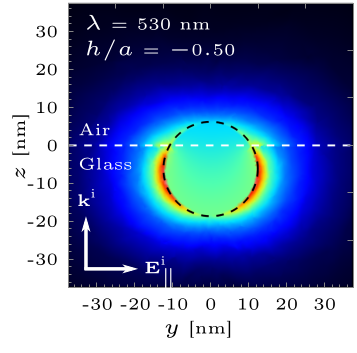
\includegraphics[width = .28\textwidth]{P-Resumen/P1.png}};
          \node[below = of Sus]{\def\svgwidth{.3\textwidth}%
          \fontsize{5}{6}%
          \includeinkscape{P-Resumen/P2-Near}};%}

        \node[flowbox, right = of Sus] (Ilu) {\fbtitle{Efecto de la iluminación}\vphantom{yÖ}
        \nodepart{two}
         \begin{minipage}{.275\textwidth}
          \begin{itemize}
          \item Partícula parcialmente embebida e incidente interna
            \begin{itemize}
            \item Onda plana $\theta_i < \theta_c$
            \item Onda evanescente $\theta_i > \theta_c$
         \end{itemize}
         \item Maximización de propiedads ópticas $\theta_i  \approx \theta_c$
        \end{itemize}
         \end{minipage}
        };

%         \node[below = of Ilu] {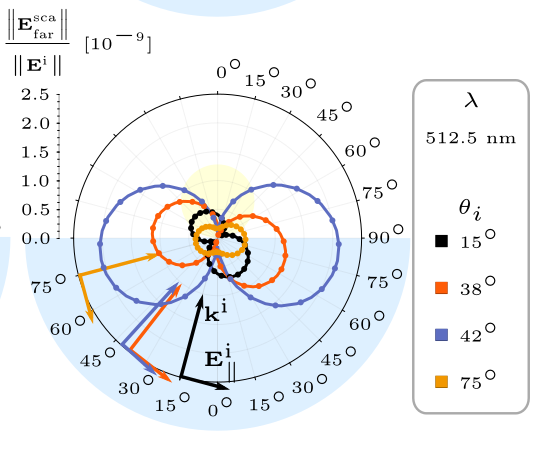
\includegraphics[width = .28\textwidth]{P-Resumen/P2.png}};
          \node[below = of Ilu]{\renewcommand{\newcirc}{{\scaleobj{.7}{\circ}}}%
          \def\svgwidth{.3\textwidth}%
          \fontsize{4.5}{5.5}%
          \includeinkscape{P-Resumen/P4-5-Far-XY-P}};%}

        \node[flowbox, right = of Ilu] (Inc) {\fbtitle{Efecto de la incrustación}\vphantom{yÖ}
        \nodepart{two}
         \begin{minipage}{.3\textwidth}
          \begin{itemize}
            \item Corrimiento al rojo (LSPR)
            \item Aumento de la extinción
            \item Pol. \textit{s}:
            \begin{itemize}
              \item Proceso homogéneo
            \end{itemize}
            \item Pol. \textit{p}:
                        \begin{itemize}
              \item $h/a$ y $\theta_i$
            \end{itemize}
          \end{itemize}\end{minipage}
        };

%         \node[below = of Inc] {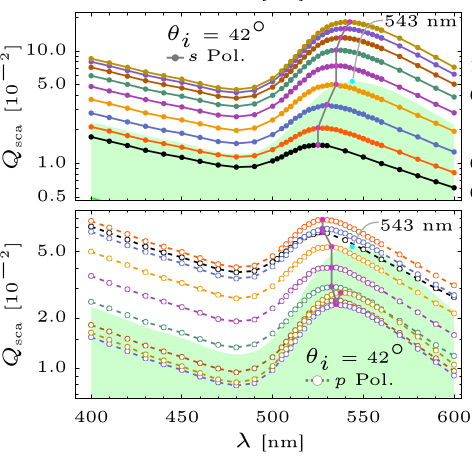
\includegraphics[width = .28\textwidth]{P-Resumen/P3.png}};
          \node[below = of Inc]{\renewcommand{\newcirc}{{\scaleobj{.625}{\circ}}}%
          \def\svgwidth{.275\textwidth}%
          \fontsize{4}{5}%
          \includeinkscape{P-Resumen/P2-Oblique-Inc-Abs}};%}

        \end{tikzpicture}
        \end{center}
      \end{frame}
